% This file was created with tikzplotlib v0.10.1.
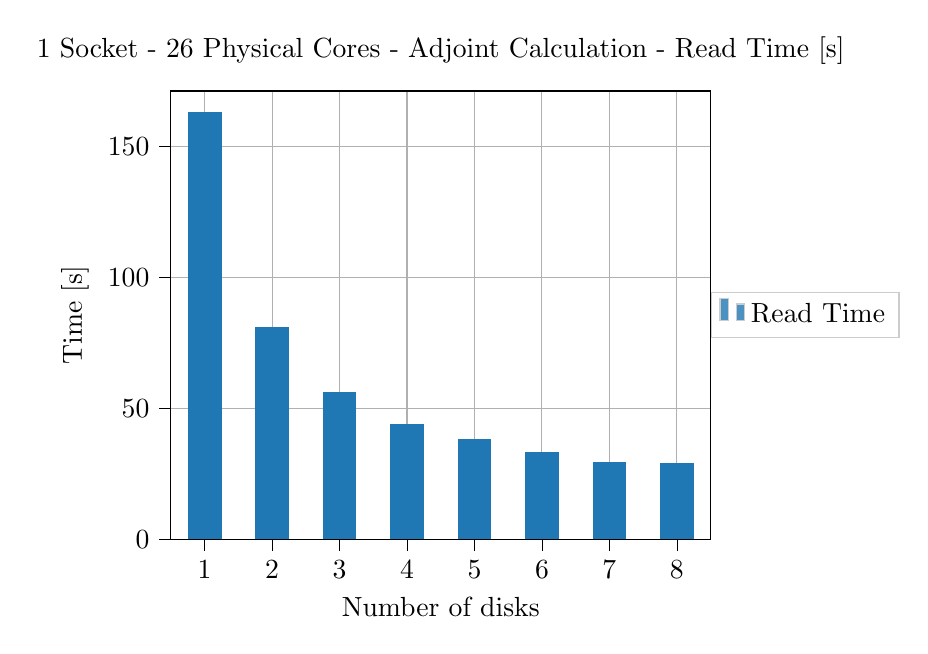
\begin{tikzpicture}

\definecolor{darkgray176}{RGB}{176,176,176}
\definecolor{lightgray204}{RGB}{204,204,204}
\definecolor{steelblue31119180}{RGB}{31,119,180}

\begin{axis}[
legend cell align={left},
legend style={
  fill opacity=0.8,
  draw opacity=1,
  text opacity=1,
  at={(1,0.5)},
  anchor=west,
  draw=lightgray204
},
tick align=outside,
tick pos=left,
title={1 Socket - 26 Physical Cores - Adjoint Calculation - Read Time [s]},
x grid style={darkgray176},
xlabel={Number of disks},
xmajorgrids,
xmin=-0.5, xmax=7.5,
xtick style={color=black},
xtick={0,1,2,3,4,5,6,7},
xticklabels={1,2,3,4,5,6,7,8},
y grid style={darkgray176},
ylabel={Time [s]},
ymajorgrids,
ymin=0, ymax=171.2865,
ytick style={color=black}
]
\draw[draw=none,fill=steelblue31119180] (axis cs:-0.25,0) rectangle (axis cs:0.25,163.13);
\addlegendimage{ybar,ybar legend,draw=none,fill=steelblue31119180}
\addlegendentry{Read Time}

\draw[draw=none,fill=steelblue31119180] (axis cs:0.75,0) rectangle (axis cs:1.25,80.95);
\draw[draw=none,fill=steelblue31119180] (axis cs:1.75,0) rectangle (axis cs:2.25,56.4);
\draw[draw=none,fill=steelblue31119180] (axis cs:2.75,0) rectangle (axis cs:3.25,44.06);
\draw[draw=none,fill=steelblue31119180] (axis cs:3.75,0) rectangle (axis cs:4.25,38.16);
\draw[draw=none,fill=steelblue31119180] (axis cs:4.75,0) rectangle (axis cs:5.25,33.29);
\draw[draw=none,fill=steelblue31119180] (axis cs:5.75,0) rectangle (axis cs:6.25,29.35);
\draw[draw=none,fill=steelblue31119180] (axis cs:6.75,0) rectangle (axis cs:7.25,29.09);
\end{axis}

\end{tikzpicture}
